\chapter{Brève description d'une page}

\section{Blocs}

\begin{figure}
    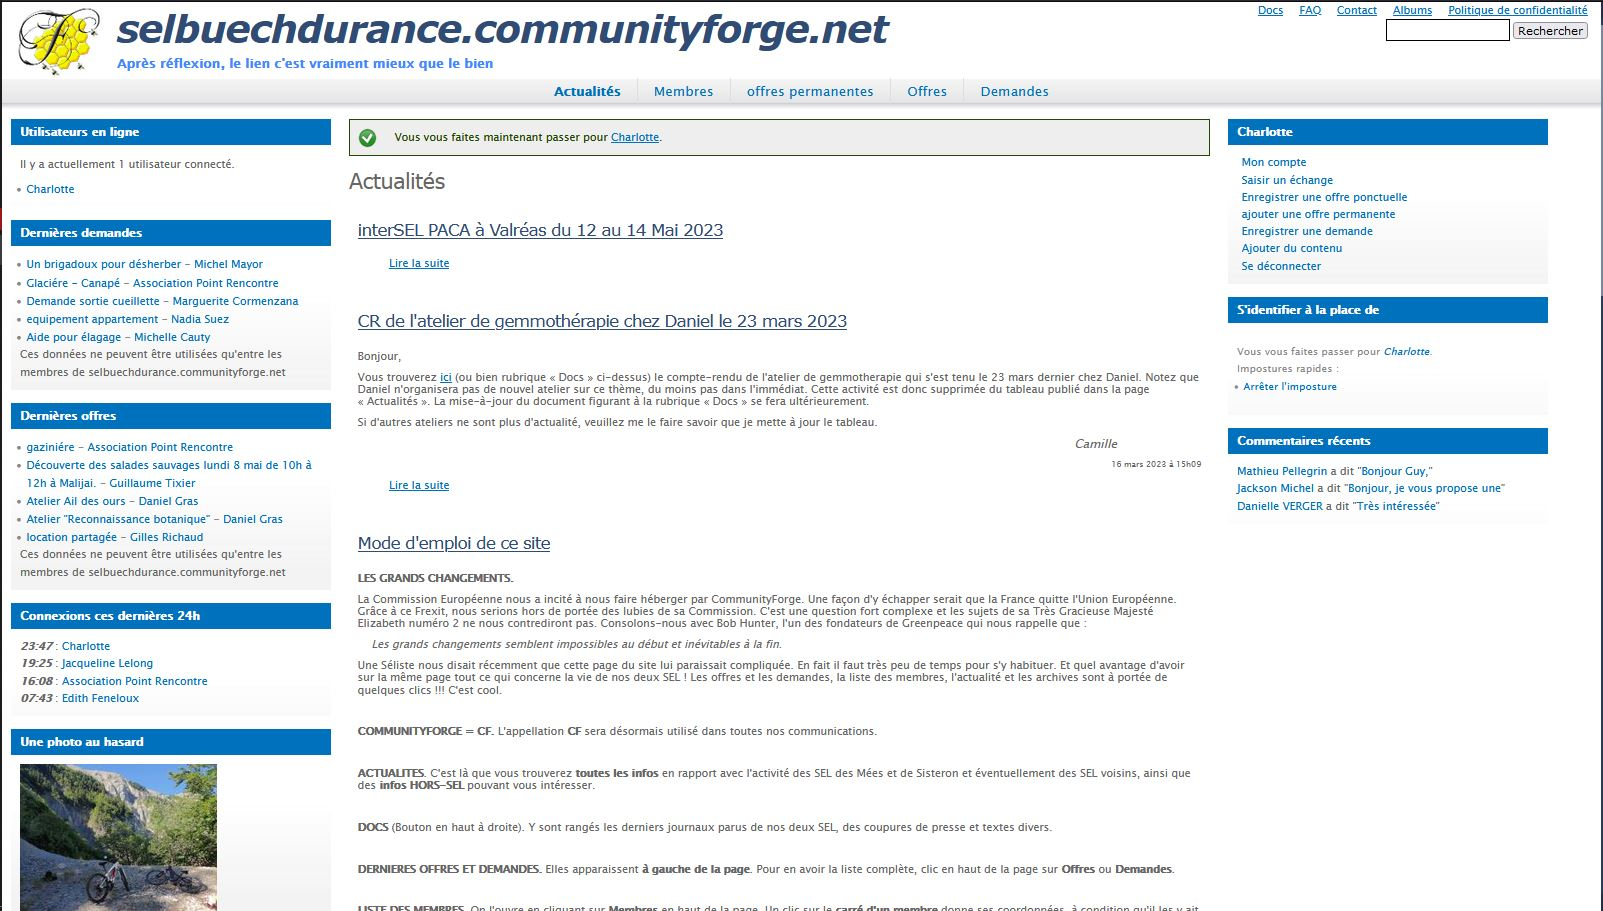
\includegraphics[width=\linewidth]{100-les_blocs_d_une_page}
    \caption[Vue générale d’une page]{Vue générale d’une page. \textsl{\small Note: Depuis cette capture d'écran, l'ordre des blocs de la colonne de gauche a été légèrement modifié (voir texte pour l'ordre actuel).}}
    \label{fig:vueGeneralePage}
\end{figure}

La figure \ref{fig:vueGeneralePage} (\vpageref{fig:vueGeneralePage}) montre le début de la page d'accueil du site \CF. Elle est constituée de différents blocs que nous allons décrire brièvement dans ce chapitre puis plus longuement pour la plupart d’entre eux dans les chapitres suivants.

\subsec{Haut de la page}

Tout en haut, à gauche, on trouve le logo du site%
%%%
\footnote{Le C et le F entrelacés avec les abeilles est un des logos par défaut des sites \CF. Il pourrait être changé pour un logo spécifique au \CdS{} si cela inspire un membre artiste !},
%%%
son nom --- en fait, son adresse internet ---, et son slogan, au centre le menu principal\index{menu principal} et à droite un petit menu secondaire\index{menu secondaire} et un champ de recherche\index{bloc!de recherche}.

\subsec{Colonne de gauche}

La colonne de gauche comporte cinq blocs: 
\begin{enumerate}
    \item dernières demandes;\index{demandes!liste des dernières}
    \item dernières offres;\index{offres!liste des dernières}
    \item utilisateurs en ligne;\index{utilisateurs!en ligne}
    \item connexions ces dernières 24 h;\index{utilisateurs!connectés ces dernières 24 h}
    \item une photo au hasard.\index{photo!au hasard}
\end{enumerate}

\subsec{Colonne de droite}

La colonne de droite comporte deux (ou trois) blocs: 
\begin{enumerate}
    \item un bloc dont le titre est le nom de l’utilisateur (ici Charlotte\footnote{Le titre sera Charlotte \textsc{Arnaud} lorsque son profil sera complété (voir note de bas de page n°\thenoteProfilPasAJour, p. \pageref{page:profilPasAJour})}; voir aussi Fig. \ref{fig:menuUtilisateur}, p. \pageref{fig:menuUtilisateur});\index{menu utilisateur}
    \item commentaires récents:\index{commentaires!liste des derniers}
    \item parfois, il pourra aussi y avoir un bloc sondage sur lequel je reviendrai.\index{sondage}
\end{enumerate}

\rem{J'ai omis le bloc \noncliquables{S’identifier à la place de}, le deuxième  dans la colonne, car il n’apparaîtra pas chez vous, ni le message \noncliquables{Vous vous faites maintenant passer pour Charlotte} en haut du bloc central%
%%%
\footnote{Un administrateur local peut s'identifier en tant qu'un autre membre --- ici, je me fais passer pour Charlotte ce qui me permet d'effectuer les actions décrites dans ce tutoriel comme si j'étais elle et non pas en tant qu'administrateur local. Ceci est parfois utile pour porter assistance à un(e) adhérent(e).}.}
%%%

\subsec{Bloc central}

Enfin, au centre de cette page d'accueil, on trouve le grand bloc \noncliquables{Actualités}.\index{bloc!Actualités@Actualités}

À la différence du contenu des colonnes gauche et droite, généralement inchangé d'une page à l'autre, le bloc central varie au gré de la navigation sur le site.


%\medskip

\section{Menus permanents}

Trois menus sont dits permanents, \cad{} qu’ils sont présents sur la plupart des pages\,:
\begin{enumerate}
    \item menu principal\;
    \item menu secondaire\;
    \item menu utilisateur.
\end{enumerate}

\subsection{Menu principal}\index{menu principal}

\begin{figure}
    
\includegraphics[width=\linewidth]{110-menu_principal}
    \caption{Menu principal}
    \label{fig:menuPrincipal}
\end{figure}
Le menu principal (Fig. \ref{fig:menuPrincipal}) est situé sous le slogan du \sel{} naguère réécrit par Arno: \noncliquables{\emph{Après réflexion, le lien c’est vraiment mieux que le bien.}} Il comporte les liens suivants:\index{menu principal!liens du} \liensmenu{Actualités}, \liensmenu{Membres}, \liensmenu{offres permanentes}, \liensmenu{Offres}, et \liensmenu{Demandes}.
\begin{figure}
    
\includegraphics[width=\linewidth]{120-menu_secondaire}
    \caption{Menu secondaire}
    \label{fig:menuSecondaire}
\end{figure}

\subsection{Menu secondaire\label{sec:menuSecondaire}}\index{menu secondaire}

Le menu secondaire (Fig. \ref{fig:menuSecondaire}, \vpageref{fig:menuSecondaire}) est situé tout en haut à droite --- au-dessus de l’outil de recherche, si vous ne l’avez pas supprimé (voir section <<~Supprimer l’affichage de certains blocs~>>, p. \pageref{sec:supprimerBlocs}). Il comporte les liens suivants:\index{menu secondaire!liens du} \liensmenu{Docs}, \liensmenu{FAQ}, \liensmenu{Contact}, \liensmenu{Albums}, et \liensmenu{Politique de confidentialité}.

\subsection{Menu utilisateur}\label{sec:menuUtilisateur}\index{menu utilisateur}

Le menu utilisateur (Fig. \ref{fig:menuUtilisateur}) 
est situé dans la colonne de droite, en général --- \cad{} lorsqu'il n'y a pas de sondage en cours --- juste au-dessous du bandeau du menu principal. Le titre du menu utilisateur est le nom de l’adhérent(e) (ici, Charlotte\footnote{Le profil de Charlotte n'était pas à jour au moment de cette capture d'écran et d'autres dans ce chapitre (voir note de bas de page n° \thenoteProfilPasAJour, page \pageref{page:profilPasAJour}).}).

Lorsqu'un sondage est en cours, il prend la place du menu utilisateur qui est alors décalé au-dessous du sondage (voir Fig. \ref{fig:sondage}, p. \pageref{fig:sondage}).

Le menu utilisateur comporte les liens suivants:\index{menu utilisateur!liens du} \liensmenu{Mon compte},
\liensmenu{Saisir un échange}, \liensmenu{Enregistrer une offre ponctuelle}, \liensmenu{ajouter une offre permanente}, \liensmenu{Enregistrer une demande}, \liensmenu{Ajouter du contenu} et \liensmenu{Se déconnecter}.
\begin{figure}
    \centering
    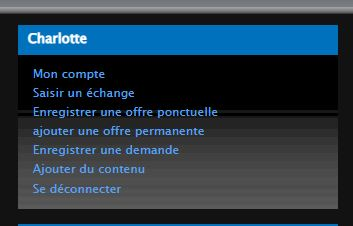
\includegraphics[width=.9\linewidth]{130-menu_utilisateur}
    \caption{Menu utilisateur}
    \label{fig:menuUtilisateur}
\end{figure}

\section{Menus contextuels}\index{menu contextuel!definition@définition}

Il existe d’autres menus qui, contrairement aux menus permanents, ne sont présents que sur certaines pages, \cad{} en fonction du contexte. Nous verrons ces menus dits contextuels dans la suite du tutoriel.

\section{Autres liens}\label{page:autresLiens}

Outre les liens des différents menus que nous venons de voir, de nombreux autres éléments sont clicables qui peuvent être utiles, \ex, le nom ainsi que le numéro d'un membre sont clicables, ils amènent à sa page de profil ce qui permet, entre autres, de lui envoyer un message (voir p. \pageref{page:envoyerCourrielMembre}); de nombreux autres éléments clicables, par contre, n’ont pas grande utilité%
%%%
\footnote{Ainsi, cliquer sur le titre d'une annonce affichera simplement celle-ci sans la mise en forme.}.
